\documentclass{article}
\usepackage{tikz}
\usetikzlibrary{arrows.meta}

\begin{document}

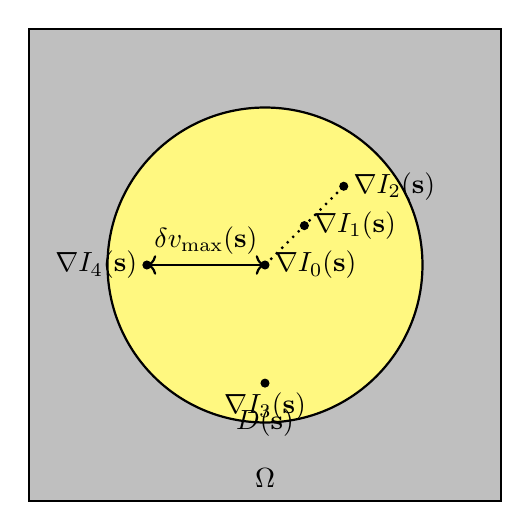
\begin{tikzpicture}
    % Define the image domain (square)
    \fill[gray!50] (0,0) rectangle (6,6);
    
    % Define the region D(s)
    \fill[yellow!50] (3,3) circle (2);
    
    % Draw the border of the image domain
    \draw[thick] (0,0) rectangle (6,6);
    
    % Draw the border of D(s)
    \draw[thick] (3,3) circle (2);
    
    % Place the gradient vectors and labels
    \filldraw (3,3) circle (0.05) node[right] {$\nabla I_0(\mathbf{s})$};
    \filldraw (3.5,3.5) circle (0.05) node[right] {$\nabla I_1(\mathbf{s})$};
    \filldraw (4,4) circle (0.05) node[right] {$\nabla I_2(\mathbf{s})$};
    \filldraw (1.5,3) circle (0.05) node[left] {$\nabla I_4(\mathbf{s})$};
    \filldraw (3,1.5) circle (0.05) node[below] {$\nabla I_3(\mathbf{s})$};
    
    % Draw the dotted line between I0 and I2
    \draw[dotted, thick] (3,3) -- (4,4);
    
    % Draw the double-headed arrow for delta_v_max
    \draw[<->, thick] (1.5,3) -- (3,3) node[midway, above] {$\delta v_{\max}(\mathbf{s})$};
    
    % Add the labels for D(s) and Omega
    \node at (3,1) {$D(\mathbf{s})$};
    \node at (3,0.3) {$\Omega$};
\end{tikzpicture}

\end{document}